% Wersja robocza wygenerowana przez Claude (2026-11-08) na prośbę zespołu; do przepisania własnymi słowami.
% Użycie AI ujawnić w preprincie. Odwołania do eksperymentów (E##) są tylko w komentarzach.
\documentclass[10pt,a4paper]{article}
\usepackage{iftex}
\ifXeTeX
  \usepackage{fontspec}
\else
  \usepackage[T1]{fontenc}
  \usepackage[utf8]{inputenc}
  \usepackage{lmodern}
\fi
\usepackage[polish]{babel}
\usepackage[margin=2.2cm]{geometry}
\usepackage{graphicx,booktabs,amsmath,xcolor,enumitem,microtype}
\usepackage[hidelinks]{hyperref}
\usepackage[most]{tcolorbox}
\usepackage[font=small,labelfont=bf]{caption}
\newcommand{\capdet}[1]{\par\footnotesize\color{black!75}#1}
\setlist{nosep,leftmargin=1.4em}
\newcommand{\x}[1]{$\times$#1}
\newcommand{\todo}[1]{\textcolor{red!70!black}{\textbf{TODO:} #1}}

\title{Szacowanie ukrytych wyświetleń postów z reakcji:\\przeniesienie modelu między platformami}
\author{Zespół projektu AMC, Politechnika Wrocławska}
\date{wersja robocza, \today}

\begin{document}
\maketitle

% ---------- roboczy spis treści: usunąć przed oddaniem ----------
\begin{tcolorbox}[colback=yellow!8,colframe=yellow!50!black,title={Roboczy spis treści (usunąć przed oddaniem)},fonttitle=\bfseries\small,fontupper=\small]
\begin{enumerate}[leftmargin=1.6em]
  \item \textbf{Wstęp} --- problem, literatura, pytanie, wkład.
  \item \textbf{Dane} --- skąd prawda na każdej platformie; Tabela~1, Rys.~1.
  \item \textbf{Metoda} --- miara błędu, walidacja po markach, dwa modele, przedziały.
  \item \textbf{Wyniki} --- Rys.~2 (wynik główny), Rys.~3 (na czym uczyć), Rys.~4 (czego model potrzebuje), Rys.~5 (kto jest źle szacowany), przedziały.
  \item \textbf{Co nie działa} --- Rys.~6: wszystkie sprawdzone metody.
  \item \textbf{Zastosowania} (1 str.) --- Rys.~7: alert, ranking marek, EMV, posty odstające.
  \item \textbf{Ograniczenia i rekomendacje}.
\end{enumerate}
\end{tcolorbox}
% ----------------------------------------------------------------

\section{Wstęp}

Firmy monitorujące media, takie jak Brand24, raportują klientom, ile osób mogło zobaczyć wzmiankę o ich marce.
Najprostsza miara zasięgu, liczba wyświetleń, często nie jest jednak widoczna: platformy ograniczają to, co pokazują
publicznie, a zakres tych danych zmienia się między platformami, formatami postów i w czasie. W praktyce zasięg
przybliża się więc stałym mnożnikiem liczby obserwujących lub reakcji, który nie mówi, jak bardzo może się mylić.

Przewidywanie popularności treści jest szeroko badane~\cite{tatar2014}, także między serwisami:
Shulman i in.~\cite{shulman2016} przenoszą model między zbiorami muzyki, książek, zdjęć i linków, a Roy
i in.~\cite{roy2013} wiedzę z Twittera na filmy z YouTube. Prace te oceniają jednak model tam, gdzie wynik jest znany.
Nie znaleźliśmy pracy, która sprawdza oszacowanie wyświetleń z reakcji na platformach, gdzie wyświetlenia są ukryte,
wobec niezależnie zmierzonej prawdy.

Pytamy, czy wyświetlenia posta na Facebooku i Instagramie da się oszacować z jego reakcji modelem uczonym wyłącznie na
innych platformach, i z jaką niepewnością. Nasz wkład:
\begin{itemize}
  \item model uczony tylko na X i YouTube szacuje wyświetlenia filmów na Facebooku z typowym błędem \x{2,4}, a rolek na
        Instagramie \x{2,65}, tak samo dobrze jak model uczony na samej platformie docelowej;
  \item pokazujemy, kiedy to przeniesienie działa (reakcje odczytane razem z wyświetleniami) i kiedy zawodzi;
  \item dla każdego posta podajemy przedział niepewności, trafny także przy brakujących danych;
  \item pokazujemy zastosowania: alert o wybiciu, ranking marek i wartość medialną.
\end{itemize}

\section{Dane}

Korzystamy z 12\,500 wzmianek o 348 markach z pięciu platform, udostępnionych przez Brand24 (po 2\,500 na platformę,
85\% z IV--VIII 2026, 85\% po angielsku). Dla TikToka, YouTube i X wyświetlenia są w eksporcie. Dla Facebooka
i Instagrama ich nie ma, więc pobraliśmy je własnym sposobem razem z reakcjami z tego samego momentu: 402 filmy z 20
marek na Facebooku i \todo{IG po partii 3:} 338 rolek z 11 marek na Instagramie. Zwykłe posty na tych platformach nie
mają licznika wyświetleń, więc wyniki dotyczą tylko filmów i rolek. Typ i sentyment wzmianek oznaczyły modele językowe,
a następnie członek zespołu je sprawdził i poprawił.

\begin{table}[!htb]
\centering\small
\caption{Dane według platformy.}
\label{tab:data}
\begin{tabular}{lrlrrr}
\toprule
Platforma & Marki & Źródło wyświetleń & Posty z wyświetleniami & Mediana wyśw. & Wyśw. na lajk \\
\midrule
TikTok    & 266 & eksport Brand24       & 2\,491 & 729    & 25 \\
YouTube   & 273 & eksport Brand24       & 2\,441 & 433    & 26 \\
X         & 252 & eksport Brand24       & 1\,803 & 27     & 22 \\
Facebook  & 20  & własny odczyt (filmy) & 402    & 1\,413 & 35 \\
Instagram & 11  & własny odczyt (rolki) & 338    & 506    & 49 \\
\bottomrule
\end{tabular}
\end{table}

\begin{figure}[!htb]
\centering
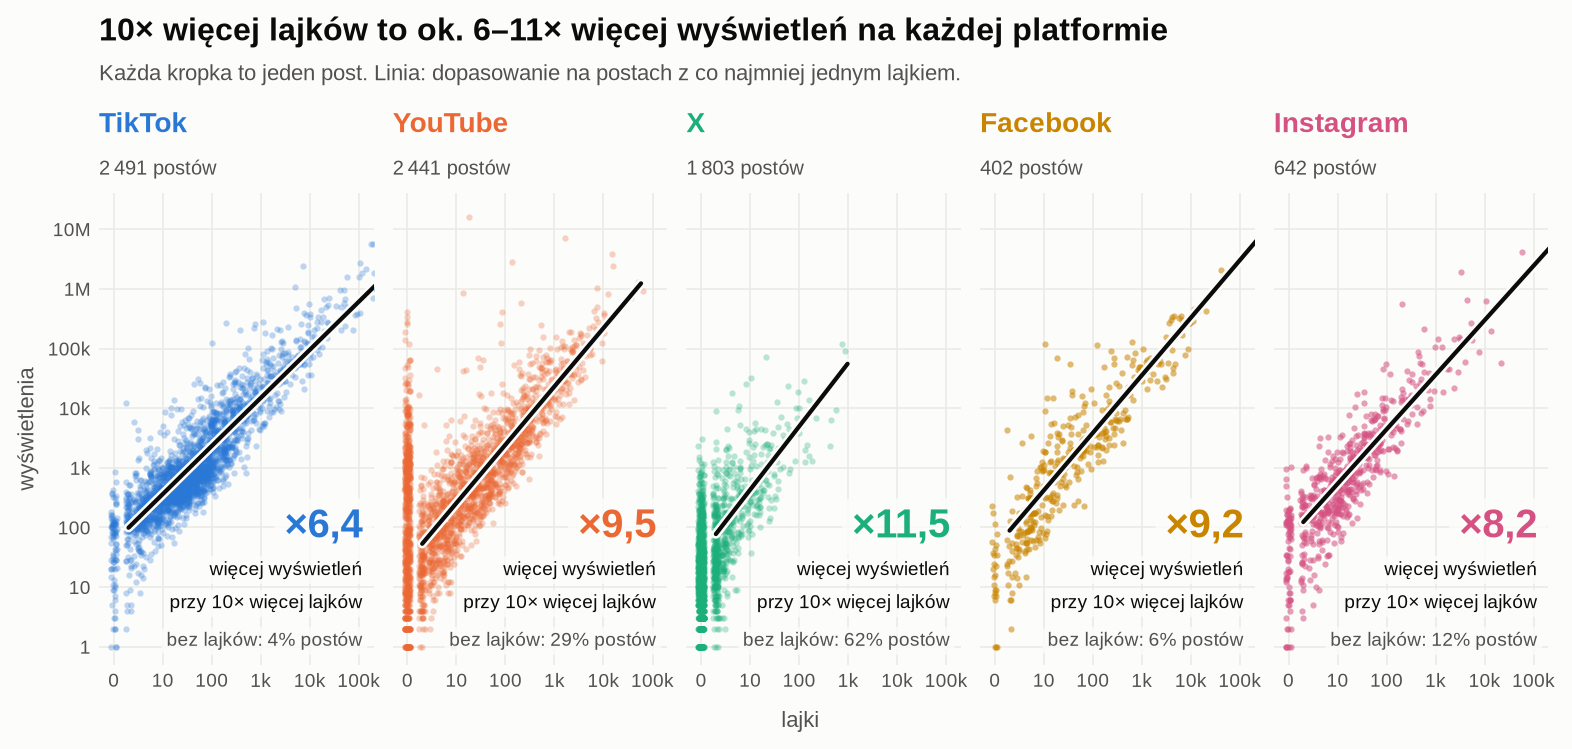
\includegraphics[width=\textwidth]{fig/data_overview_pl.png}
\caption{Wyświetlenia a lajki, osobno dla każdej platformy.
\capdet{Obie osie w skali logarytmicznej; posty bez lajków przy zerze. Linia: prosta dopasowana na postach z co najmniej
jednym lajkiem; liczba: ile razy więcej wyświetleń ma post z 10 razy większą liczbą lajków. TikTok, YouTube, X: eksport
Brand24; Facebook (filmy), Instagram (rolki): nasz odczyt.}}
\label{fig:data}
\end{figure}

\section{Metoda}

Przewidujemy $y=\log_{10}(\text{wyświetlenia})$. Błąd podajemy jako MAE w tej skali i jako mnożnik
$10^{\text{MAE}}$ (MAE 0,30 $\approx$ \x{2}). Wszystkie modele oceniamy pięciokrotną walidacją krzyżową z podziałem po
markach, więc każda ocena dotyczy marki, której model nie widział; przedziały ufności liczymy bootstrapem po markach.
Na TikToku, YouTube i X używamy CatBoost~\cite{catboost} na obserwujących, reakcjach i flagach braków. Do przeniesienia
na Facebooka i Instagram używamy regresji ridge na $\log(1+\text{lajki})$ i $\log(1+\text{komentarze})$, czyli dwóch
polach, które ma każda platforma, uczonej na X i YouTube razem; przy pominiętej platformie przenosi się ona lepiej niż
CatBoost. Przedziały 50\% i 90\% dla każdego posta dają konformalna regresja kwantylowa~\cite{romano2019}.
% E114, E124, E61/E131 (ridge > CatBoost przy pominiętej platformie), E118, E137.

\section{Wyniki}

\paragraph{Wynik główny.} Rys.~\ref{fig:main} zestawia oba scenariusze. Na TikToku, YouTube i X, gdzie model uczy
się na tej samej platformie, typowy błąd wynosi \x{1,9}, \x{2,9} i \x{3,0}. Na Facebooku i Instagramie model nie widział
ani jednego posta z tych platform, a myli się \x{2,43} (przedział ufności \x{2,05}--\x{3,03}) i \x{2,65}
(\x{2,39}--\x{3,12}). To tyle samo, co ten sam model uczony na samej platformie docelowej (\x{2,42} i \x{2,36}), więc
zależność między reakcjami a wyświetleniami przenosi się między platformami prawie bez straty. Kolejność postów jest
zachowana bardzo dobrze (Spearman 0,91 i 0,88).
% results_a/results_b_numbers.json; CI MAE 0,312-0,482 i 0,379-0,494.

\begin{figure}[!htb]
\centering
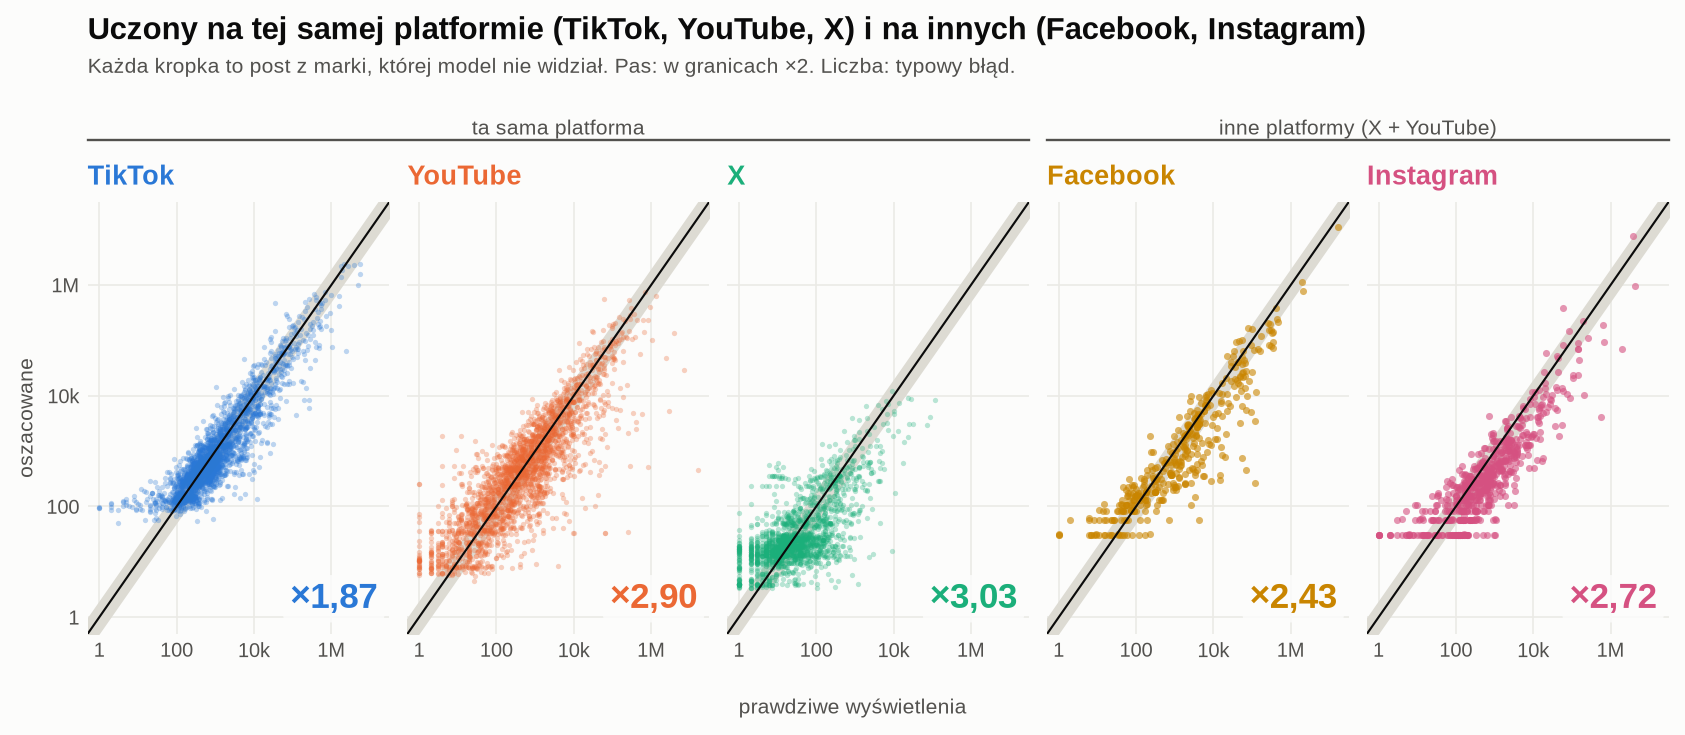
\includegraphics[width=\textwidth]{fig/preprint_main_pl.png}
\caption{Oszacowane a prawdziwe wyświetlenia.
\capdet{Każda kropka to jeden post, oszacowany przez model, który nie widział jego marki (walidacja krzyżowa po
markach). TikTok, YouTube, X: CatBoost na obserwujących, reakcjach i flagach braków, uczony na tej samej platformie;
prawda z eksportu Brand24. Facebook (402 filmy, 20 marek), Instagram (338 rolek, 11 marek): ridge na $\log$ lajków
i komentarzy uczony tylko na X i YouTube; prawda z naszego odczytu. Szary pas: oszacowanie w granicach \x{2}. Liczba:
typowy błąd $10^{\text{MAE}}$.}}
\label{fig:main}
\end{figure}

\paragraph{Na czym uczyć.} Facebook i Instagram dają się oszacować z dowolnej platformy z błędem \x{2,4}--\x{3,1}
(Rys.~\ref{fig:combos}). Wyjątkiem jest X: model uczony na X myli się na YouTube \x{5,5}, a modele uczone gdzie indziej
mylą się na X \x{3,6}--\x{4,6}. Na X większość postów ma zero lub jeden lajk (Rys.~\ref{fig:data}), więc reakcje
mówią tam mało. Więcej platform w treningu nie zawsze pomaga: wszystkie cztery pozostałe dają na X \x{4,4}, a sam
Facebook \x{3,6}.
\todo{później: szósta platforma z publicznymi wyświetleniami (backlog B30).}

\begin{figure}[!htb]
\centering
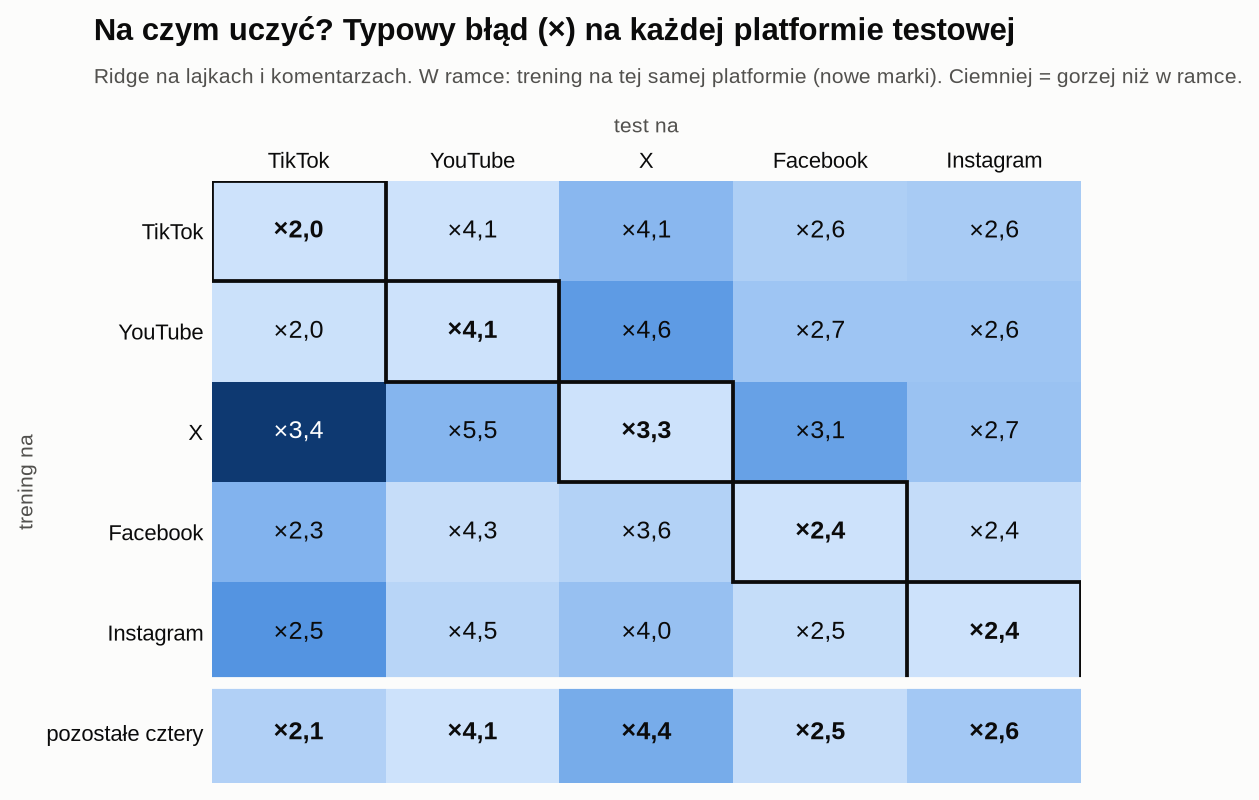
\includegraphics[width=.68\textwidth]{fig/train_combos_simple_pl.png}
\caption{Typowy błąd przy uczeniu na jednej platformie i teście na innej.
\capdet{Ridge na $\log$ lajków i komentarzy (jedyne dwa pola, które ma każda platforma). Wiersz: platforma treningowa,
ostatni wiersz: wszystkie cztery pozostałe naraz. Kolumna: platforma testowa. W ramce: trening i test na tej samej
platformie, na markach spoza treningu. Kolor: o ile błąd jest większy niż w ramce danej kolumny.}}
\label{fig:combos}
\end{figure}

\paragraph{Czego model potrzebuje.} Przeniesienie działa tylko z lajkami odczytanymi razem z wyświetleniami
(Rys.~\ref{fig:needs}A). Same komentarze dają \x{6,2}--\x{7,4}, a lajki i komentarze z eksportu, odczytane w innym
momencie niż wyświetlenia, \x{6,8}. Na platformach ze znanymi wyświetleniami (Rys.~\ref{fig:needs}B) brak obserwujących
prawie nie szkodzi, a brak reakcji podnosi błąd do \x{3,8}--\x{5,2}. Dla każdego układu dostępnych pól uczymy osobny
model z osobnym przedziałem, dzięki czemu przedział 90\% trafia w 88--90\% postów w każdym przypadku; model uczony na
pełnych danych i karmiony niepełnymi trafiałby tylko w 46--83\%.
% E177, E176, results_b (comments only).

\begin{figure}[!htb]
\centering
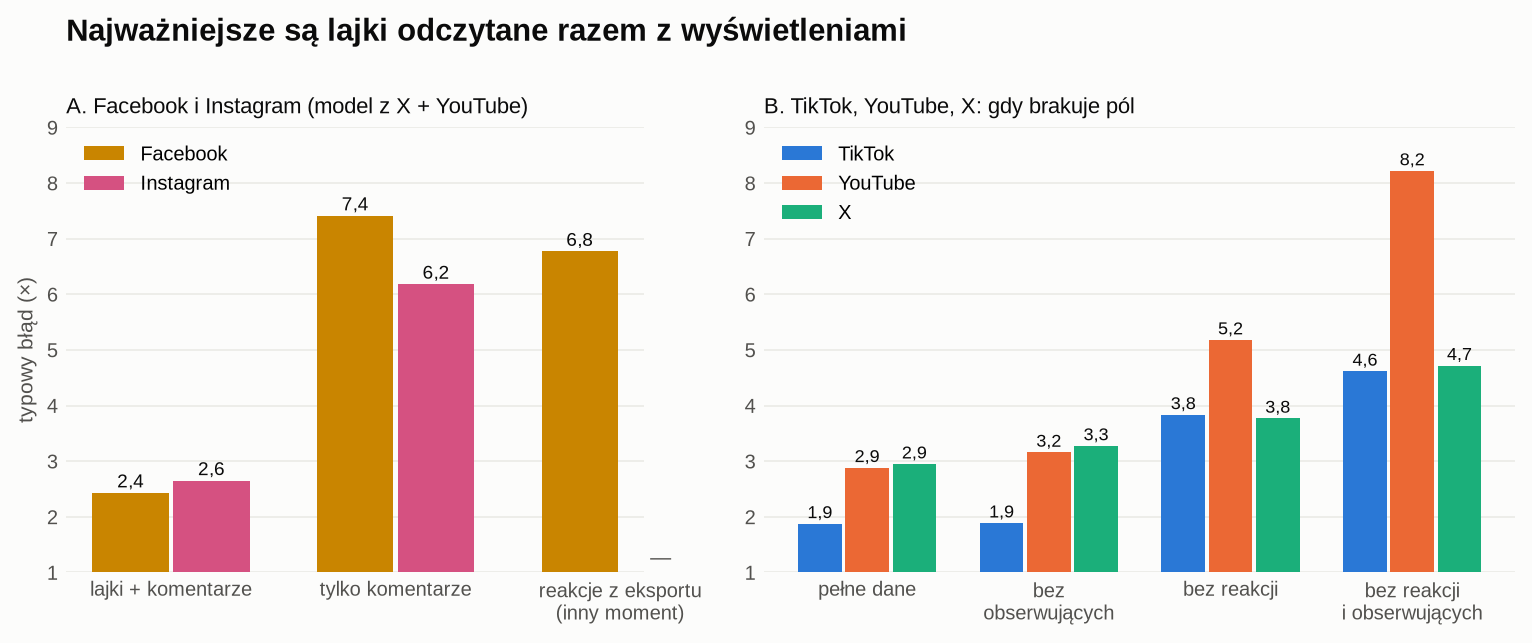
\includegraphics[width=\textwidth]{fig/preprint_needs_pl.png}
\caption{Typowy błąd przy różnych danych wejściowych.
\capdet{A: Facebook i Instagram, ridge uczony na X i YouTube. ,,Lajki + komentarze'': nasze pola odczytane razem
z wyświetleniami; ,,tylko komentarze'': model na samych komentarzach; ,,reakcje z eksportu'': lajki i komentarze
z eksportu Brand24, odczytane w innym momencie niż wyświetlenia (dla Instagramu brak). B: TikTok, YouTube, X, osobny
CatBoost dla każdego układu dostępnych pól, walidacja po markach.}}
\label{fig:needs}
\end{figure}

\paragraph{Kto jest źle szacowany.} Na każdej platformie, także po przeniesieniu, model zawyża posty z małą liczbą
wyświetleń (ok. \x{2} poniżej 100 wyświetleń) i zaniża duże (Rys.~\ref{fig:size}). To typowe ściąganie do średniej:
reakcje nie odróżniają dobrze postu, który się wybił, od zwykłego. Najsilniej widać to na X, gdzie posty powyżej 10\,000
wyświetleń są zaniżone kilkanaście razy; po przeniesieniu Instagram zaniża duże rolki około \x{3}.

\begin{figure}[!htb]
\centering
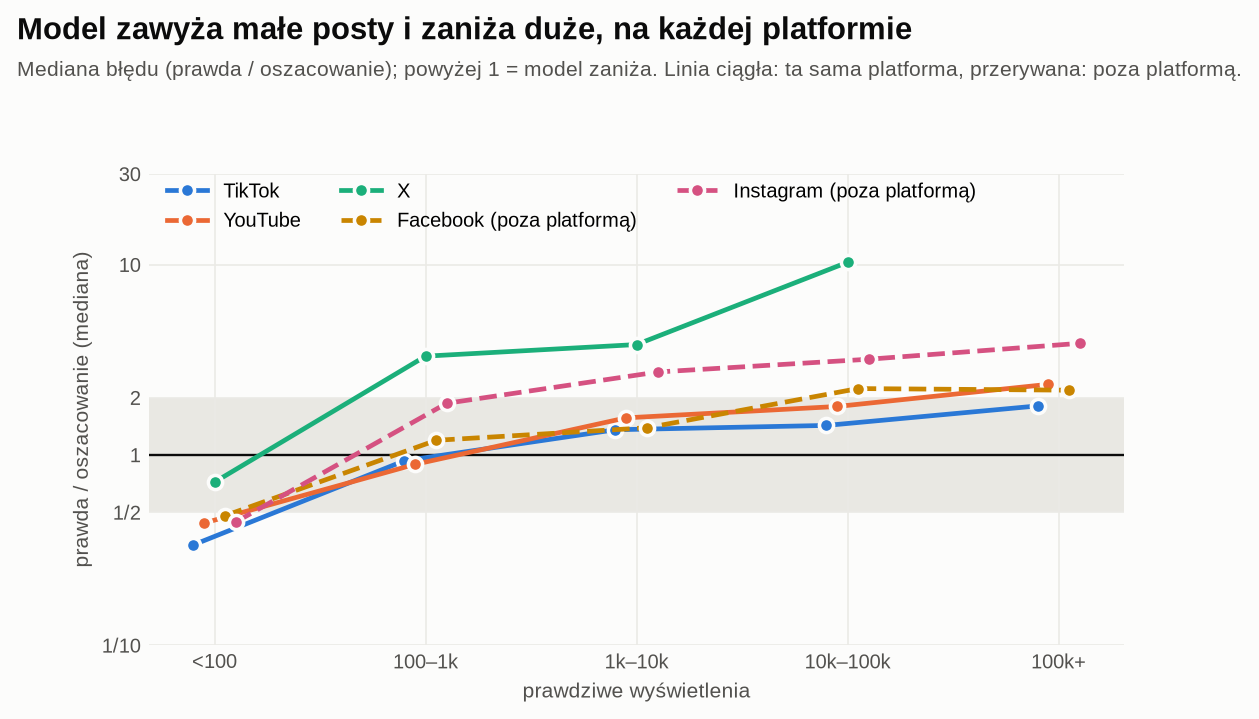
\includegraphics[width=.78\textwidth]{fig/preprint_size_pl.png}
\caption{Błąd według wielkości posta.
\capdet{Mediana stosunku prawdziwych do oszacowanych wyświetleń w przedziałach prawdziwych wyświetleń (pokazane
przedziały z co najmniej 10 postami). Powyżej 1: model zaniża. Szary pas: w granicach \x{2}. Modele jak na
Rys.~\ref{fig:main}.}}
\label{fig:size}
\end{figure}

\paragraph{Przedziały.} Przedział 90\% trafia w 89--90\% postów na TikToku, YouTube i X, także na miesiącach spoza
treningu (0,90--0,93). Na Facebooku trafia w 93\% filmów kont poniżej miliona obserwujących, ale dla największych kont
tylko w 80--86\%. Jeśli zamiast liczby podamy jeden z trzech przedziałów (<1\,000, 1\,000--10\,000, >10\,000), trafiamy
w 78--82\% postów na TikToku, YouTube, Facebooku i Instagramie.
% E118, E142, E123, E151, E199.

\section{Co nie działa}\label{sec:nie}

Sprawdziliśmy ponad dwadzieścia sposobów poprawienia modelu poza reakcjami i obserwującymi (Rys.~\ref{fig:methods}):
inne rodziny modeli, tekst (od TF-IDF po dostrojone transformery), etykiety AI, grafy autorów i marek oraz dane
zewnętrzne o markach. Żaden nie zmienia błędu o więcej niż \x{1,07}, a większość mniej niż \x{1,02} albo pogarsza wynik.
Najwięcej daje połączenie wszystkich rodzin modeli (do \x{1,07} na YouTube), ale kosztem dużo bardziej złożonego
modelu. Tekst pomaga trochę na YouTube i X, grafy i dane zewnętrzne szkodzą. Na Facebooku tekst pogarsza przeniesienie
(MAE 0,385 $\to$ 0,436). Jedyna cecha, która pomaga wyraźnie, to historia autora: dla postów autorów, których model już
widział, błąd spada o 0,10--0,15, ale takich postów jest tylko 3--16\%.
% E54, E47, E53, E50, E65, E127, E170-E175, ablacja; E100 (FB tekst); E68/E70 (autor).

\begin{figure}[!htb]
\centering
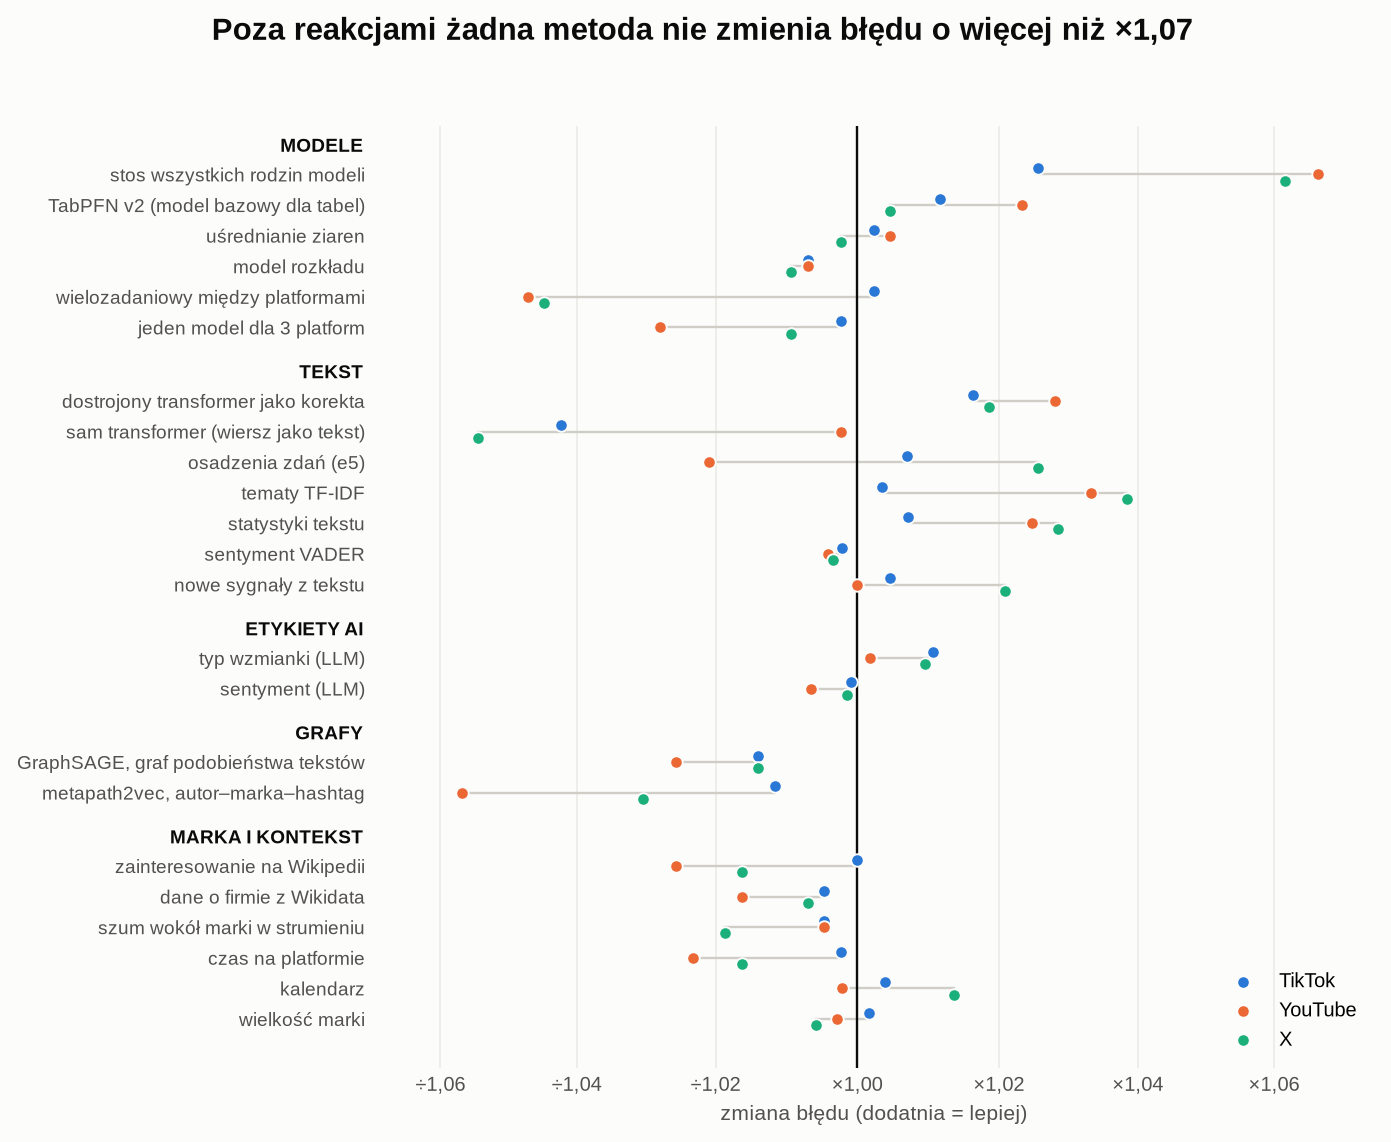
\includegraphics[width=.95\textwidth]{fig/preprint_methods_pl.png}
\caption{Wszystkie sprawdzone metody i źródła danych.
\capdet{Zmiana typowego błędu względem modelu końcowego (modele, transformery, osadzenia, grafy, dane zewnętrzne) albo
względem modelu na obserwujących i reakcjach (TF-IDF, statystyki tekstu, VADER, etykiety AI, kalendarz, wielkość marki).
W prawo: lepiej, w lewo: gorzej; $\times$1,02 to zmiana MAE o około 0,01. \emph{Stos}: średnia wszystkich rodzin modeli
na tych samych podziałach. \emph{TabPFN v2}: wstępnie wytrenowany model dla tabel. \emph{Wielozadaniowy}: jedna sieć
dla trzech platform. \emph{Transformer jako korekta}: dostrojony model językowy przewiduje błąd CatBoost z tekstu posta;
\emph{sam transformer}: cały wiersz zapisany jako tekst. \emph{Osadzenia e5}: wielojęzyczny model zdań. \emph{Etykiety
LLM}: typ i sentyment z modelu językowego. \emph{GraphSAGE}: sieć grafowa na grafie podobnych tekstów;
\emph{metapath2vec}: osadzenia grafu autor--marka--hashtag. \emph{Wikipedia, Wikidata}: zainteresowanie marką
i dane o firmie. Wszystko z walidacją po markach.}}
\label{fig:methods}
\end{figure}

\section{Zastosowania}

\begin{figure}[!htb]
\centering
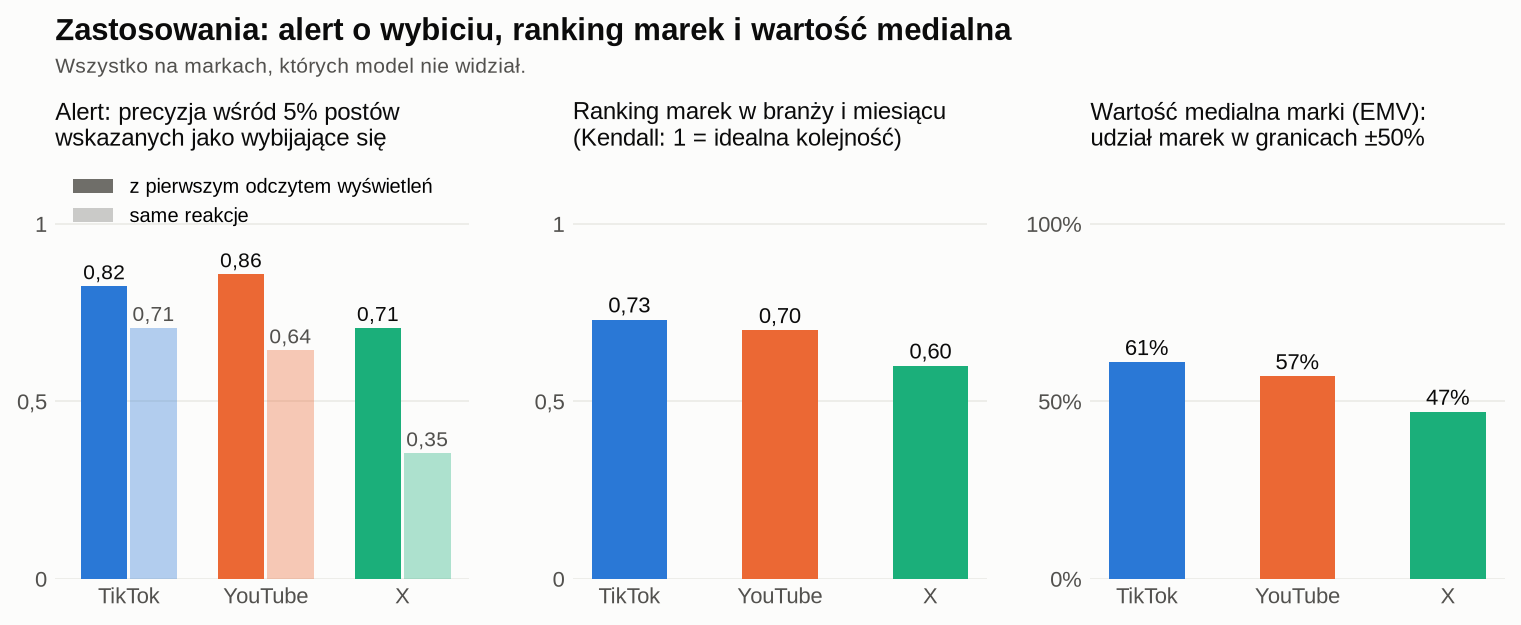
\includegraphics[width=\textwidth]{fig/preprint_side_pl.png}
\caption{Zastosowania oszacowania na TikToku, YouTube i X.
\capdet{Alert: z postów odczytanych po raz pierwszy model wskazuje 5\%, które będą miały najwięcej wyświetleń; słupek
to odsetek trafnych wskazań (289--336 postów na platformę, jeden miesiąc). Ranking: średni współczynnik Kendalla między
oszacowaną a prawdziwą kolejnością marek w parach branża--miesiąc (52 / 51 / 42 par). EMV: wyświetlenia przeliczone na pieniądze
stawką za tysiąc; odsetek marek, dla których oszacowane EMV mieści się w $\pm$50\% prawdziwego (238 / 213 / 189 marek).}}
\label{fig:side}
\end{figure}

\paragraph{Alert o wybiciu.} Z pierwszym odczytem wyświetleń model wskazuje 5\% postów, które się wybiją, z trafnością
0,82 / 0,86 / 0,71; same reakcje dają 0,71 / 0,64 / 0,35 (Rys.~\ref{fig:side}). Przy trzy razy większej liczbie
alertów łapie 82--100\% wybijających się postów.

\paragraph{Ranking marek.} Sumując oszacowane wyświetlenia marek w branży i miesiącu, odtwarzamy ich kolejność
(Kendall 0,73 / 0,70 / 0,60).

\paragraph{Wartość medialna.} EMV marki liczone z oszacowanych wyświetleń mieści się w $\pm$50\% prawdziwego dla 61\% /
57\% / 47\% marek.

\paragraph{Posty odstające.} Na TikToku posty z dużo większą liczbą wyświetleń niż wynika z reakcji to częściej
promocja (51\% wobec 34\%), a z dużo mniejszą częściej spam (26\% wobec 13\%).
% E185, E186, E188, E184.
\todo{dobić do pełnej strony: np. krzywa trafności alertu od liczby alertów, przykład rankingu jednej branży.}

\section{Ograniczenia i rekomendacje}

Wynik dla Facebooka opiera się na 20 markach (bez trzech największych \x{2,9}), a dla Instagramu na 11 (\x{2,95}).
Posty wiralowe są zaniżane \x{9}--\x{14}, więc sumy marek mylą się o więcej niż \x{2} dla 29--47\% marek. Wyniki
opisują zależności, nie przyczyny. Dostawcy monitoringu rekomendujemy: odczytywać reakcje razem z wyświetleniami,
zapisywać braki jako brak, a nie zero, robić drugi odczyt wyświetleń i przechowywać historię autorów.
% E178, E180, E202.

\todo{jeden wykres końcowy: nasz model a stały mnożnik Brand24.}
\todo{opis użycia AI zgodnie z wymaganiami kursu; odtwarzalność: repozytorium, skrypty, rejestr eksperymentów.}

\begin{thebibliography}{9}
\bibitem{tatar2014} A.~Tatar, M.~D. de~Amorim, S.~Fdida, P.~Antoniadis. A survey on predicting the popularity of web
  content. \emph{Journal of Internet Services and Applications}, 5:8, 2014.
\bibitem{shulman2016} B.~Shulman, A.~Sharma, D.~Cosley. Predictability of popularity: gaps between prediction and
  understanding. \emph{ICWSM}, 2016.
\bibitem{roy2013} S.~D. Roy, T.~Mei, W.~Zeng, S.~Li. Towards cross-domain learning for social video popularity
  prediction. \emph{IEEE Transactions on Multimedia}, 15(6), 2013.
\bibitem{catboost} L.~Prokhorenkova, G.~Gusev, A.~Vorobev, A.~V. Dorogush, A.~Gulin. CatBoost: unbiased boosting with
  categorical features. \emph{NeurIPS}, 2018.
\bibitem{romano2019} Y.~Romano, E.~Patterson, E.~Cand\`es. Conformalized quantile regression. \emph{NeurIPS}, 2019.
\end{thebibliography}

\end{document}
